\documentclass{article}
\usepackage[margin=0.75in]{geometry}
\usepackage{mymath}
\usepackage{subcaption}
\usepackage{tikz}

\title{Test Creator System Design}
\author{Nathan Gurrin-Smith}
\begin{document}
\maketitle

\section{Introduction}
This is a program that will be used to generate practice tests from a list of questions. It aims to help improve learning by encouraging frequent, interleaved testing.

\section{Use Cases}
\begin{itemize}
    \item Login
    \item Add, view, edit, and delete presets
    \item Add, view, edit, and delete questions
    \item Add, view, edit, and delete categories
    \item Generate practice tests
\end{itemize}

\section{Technology}
The framework being used is PERN (Postgres, Express, React, Node).

\subsection{Server (Node + Express)}
The main \texttt{server.js} file contains the base routes along with the middleware. Additionally, we have the following groups of modules:
\begin{itemize}
    \item Routes: used to direct requests to the right controller
    \item Controllers: manages which services are used and client responses
    \item Services: handles business logic of each task
    \item Models: handles interaction with the database
\end{itemize}

\subsubsection*{Routes}
We are using the \texttt{/api/} style. The routes file will \textbf{only} contain the HTTP method and which controller function it will use. For example:
\begin{center}
    \texttt{router.METHOD("/", Controller.Function)}
\end{center}

\subsubsection*{Controllers}
The controllers manage which services are activated when. It also handles client responses. These files are the \textbf{only} place where statements of the form \texttt{res.RESPONSE} can be put.

\subsubsection*{Services}
These modules handle the underlying business logic of each task the controller asks to be completed. These files are the \textbf{only} place where calls to the models can be put.

\subsubsection*{Models}
These modules handle individual interactions with the database. These files are the \textbf{only} place where calls to the database can be put.

\subsection{Client (React + Next.js)}
There are two main pages to the application. The first is the index page, at index.js, where users can create an account and sign in. The second is the user page, at [username].js, which is where all the user specific functions are found (see use cases above).

\subsection{Data (PostgreSQL)}
\subsubsection*{Naming Conventions}
We will use the following naming conventions for our data model
\begin{itemize}
    \item Tables and columns will be in PascalCase.
    \item Tables and columns will be singular.
    \item Junction tables will be named JunctionTable1Table2
\end{itemize}
Note: PostgreSQL automatically forces lowercase internally, but we'll always reference by PascalCase.

Note: Because of the above note, we must reference all columns with lowercase in our javascript files.

\subsubsection*{Data Model}

We will have the following data model:

\begin{figure}[h!]
    \begin{subfigure}{\textwidth}
        \begin{tabular}{|c|c|c|}
            \hline
            \multicolumn{3}{|c|}{UserAccount} \\
            \hline
            UserAccountID & Username & Password \\
            \hline
        \end{tabular}
        \vspace*{2em}
    \end{subfigure}
    \begin{subfigure}{\textwidth}
        \begin{tabular}{|c|c|c|c|c|}
            \hline
            \multicolumn{5}{|c|}{ClientAuthentication} \\
            \hline
            ClientID & LastLogin & RefreshToken & RefreshTokenExpiry & UserAccountID (FK) \\
            \hline
        \end{tabular}
        \vspace*{2em}
    \end{subfigure}
    \begin{subfigure}{\textwidth}
        \begin{tabular}{|c|c|c|c|c|c|}
            \hline
            \multicolumn{6}{|c|}{Preset} \\
            \hline
            PresetID & Name & Preamble & Sep & Postamble & UserAccountID(FK) \\
            \hline
        \end{tabular}
        \vspace*{2em}
    \end{subfigure}
    \begin{subfigure}{0.2\textwidth}
        \begin{tabular}{|c|c|}
            \hline
            \multicolumn{2}{|c|}{Collection} \\
            \hline
            CollectionID & Name \\
            \hline
        \end{tabular}
        \vspace*{2em}
    \end{subfigure}
    \begin{subfigure}{0.4\textwidth}
        \begin{tabular}{|c|c|c|}
            \hline
            \multicolumn{3}{|c|}{SubCollection} \\
            \hline
            SubCollectionID & Name & CollectionID(FK) \\
            \hline
        \end{tabular}
        \vspace*{2em}
    \end{subfigure}
    \begin{subfigure}{0.3\textwidth}
        \begin{tabular}{|c|c|c|c|c|}
            \hline
            \multicolumn{4}{|c|}{Question} \\
            \hline
            QuestionID & Name & Content & Source \\
            \hline
        \end{tabular}
        \vspace*{2em}
    \end{subfigure}
    \begin{subfigure}{0.5\textwidth}
        \begin{tabular}{|c|c|}
            \hline
            \multicolumn{2}{|c|}{JunctionUserAccountCollection} \\
            \hline
            UserAccountID(FK) & CollectionID(FK) \\
            \hline
        \end{tabular}
        \vspace*{2em}
    \end{subfigure}
    \begin{subfigure}{0.5\textwidth}
        \begin{tabular}{|c|c|}
            \hline
            \multicolumn{2}{|c|}{JunctionUserAccountPreset} \\
            \hline
            UserAccountID(FK) & PresetID(FK) \\
            \hline
        \end{tabular}
        \vspace*{2em}
    \end{subfigure}
    \begin{subfigure}{0.5\textwidth}
        \begin{tabular}{|c|c|}
            \hline
            \multicolumn{2}{|c|}{JunctionSubCollectionQuestion} \\
            \hline
            SubCollectionID(FK) & QuestionID(FK) \\
            \hline
        \end{tabular}
        \vspace*{2em}
    \end{subfigure}
    \begin{subfigure}{0.5\textwidth}
        \begin{tabular}{|c|c|}
            \hline
            \multicolumn{2}{|c|}{JunctionCollectionSubCollection} \\
            \hline
            CollectionID(FK) & SubCollectionID(FK) \\
            \hline
        \end{tabular}
        \vspace*{2em}
    \end{subfigure}
    \begin{subfigure}{\textwidth}
        \begin{tabular}{|c|c|c|}
            \hline
            \multicolumn{3}{|c|}{JunctionUserAccountQuestion} \\
            \hline
            UserAccountID(FK) & QuestionID(FK) & LastReviewed \\
            \hline
        \end{tabular}
        \vspace*{2em}
    \end{subfigure}
\end{figure}

Which are related via,
\begin{center}
    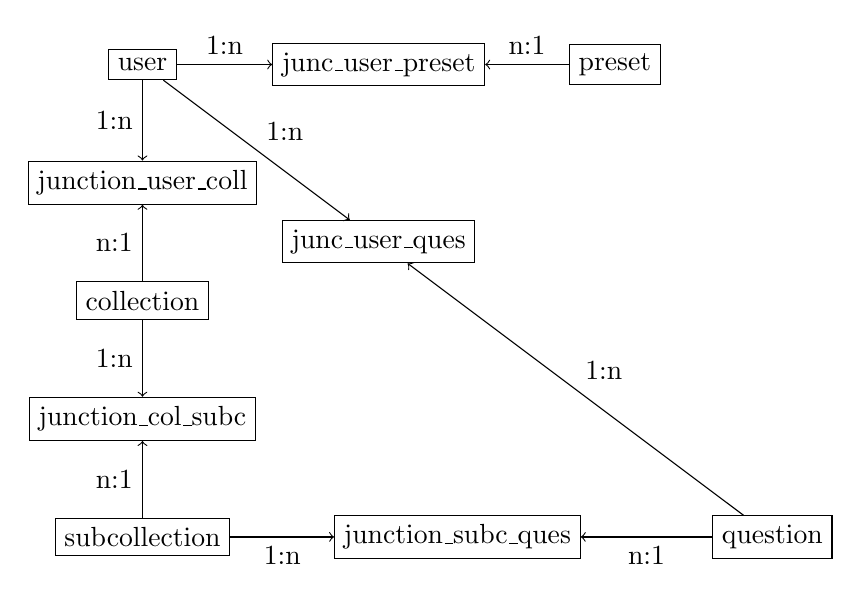
\begin{tikzpicture}
        \node[draw] at (0,0) (A) {user};
        \node[draw] at (3,0) (B) {junc\_user\_preset};
        \node[draw] at (6,0) (C) {preset};
        \node[draw] at (0,-1.5) (D) {junction\_user\_coll};
        \node[draw] at (0,-3) (E) {collection};
        \node[draw] at (0,-4.5) (F) {junction\_col\_subc};
        \node[draw] at (0,-6) (G) {subcollection};
        \node[draw] at (4,-6) (H) {junction\_subc\_ques};
        \node[draw] at (8,-6) (I) {question};
        \node[draw] at (3,-2.25) (J) {junc\_user\_ques};

        \draw [->] (A) -- (B) node[midway,above] {1:n};
        \draw [<-] (B) -- (C) node[midway,above] {n:1};
        \draw [->] (A) -- (D) node[midway,left] {1:n};
        \draw [<-] (D) -- (E) node[midway,left] {n:1};
        \draw [->] (E) -- (F) node[midway,left] {1:n};
        \draw [<-] (F) -- (G) node[midway,left] {n:1};
        \draw [->] (G) -- (H) node[midway,below] {1:n};
        \draw [<-] (H) -- (I) node[midway,below] {n:1};
        \draw [->] (I) -- (J) node[midway,above right] {1:n};
        \draw [<-] (J) -- (A) node[midway,above right] {1:n};
    \end{tikzpicture}
\end{center}

\textbf{Orphans:} Some of the properties above require a parent. These are,
\begin{itemize}
    \item A Collection requires at least one parent UserAccount,
    \item A SubCollection requires a parent Collection,
    \item A Question requires a parent UserAccount and a parent SubCollection
    \item A Preset requires a parent UserAccount
\end{itemize}
Thus, when we delete a parent, we not only need to delete entries in the junction table, but also the entries in the child tables since, most frequently, the foreign keys will be stored in the junction table and not the child table. The \texttt{cleanX} functions in the \texttt{service} modules handle this.

\subsection{Jobs}
There is a single job that runs once every day which removes all unspecified user accounts from the database. These user accounts are hardcoded into the application and can be added by the developer. The unspecified accounts are removed to keep data costs low.

\end{document}
